
\subsection{Aufsteigende motorische Bahnen}
Die aufsteigenden Bahnen des Rückenmarks leiten sensorische und propriozeptive Information an das Gehirn. Die propriozeptive Information ist dabei für die Ausführung der Motorik eine essentielle Grundlage. Die wichtigsten aufsteigenden Bahnen wurden dabei in Kapitel~\ref{sec:sensorische_Bahnen} bereits besprochen. In diesem Unterkapitel wird noch auf eine weitere Bahn eingegangen, welche wichtige Informationen an das Cerebellum zur richtigen Koordination der Bewegungen liefert. Dies ist der \textit{Tractus spinocerebellaris}. 

\subsubsection{Tractus spinocerebellaris} \index{Tractus! spinocerebellaris} \label{subsub:spinocerebellaris}
Die spinocerebellaren Trakte oder auch \textbf{Kleinhirnseitenstrangbahnen} leiten propriozeptive Informationen, die aus den Muskelspindeln, Mechanorezeptoren, wie das Golgi-Sehnenorgan, oder auch aus Tastrezeptoren stammen, zum Kleinhirn \textsuperscript{\cite[Kap.~8]{crossman2014neuroanatomy}}. Dieser Input ist wichtig für die richtige Funktion des Cerebellums. Es ist ein wichtiger Bestandteil der Bewegungskoordination und Körperhaltungskontrolle, wofür die eingehende Rückmeldung der aktuellen Körperlage notwendig ist \textsuperscript{\cite[3]{trepel2011neuroanatomie}}. Insgesamt zählen vier unterschiedliche Fasertrakte zu den Kleinhirnseitenstrangbahnen. Der dorsale und ventrale spinocerebellare Strang beziehen dabei ihre Informationen aus den unteren Extremitäten. Analog dazu gibt es den cuneocerebellaren und rostralen spinocerebellaren Fasertrakt, die Information aus den oberen Extremitäten erhalten. Der dorsale spinocerebellare Trakt entstammt aus einer Gruppe an Zellen aus dem Hinterhorn der Thorakal- und Lumbalsegmenten, auch bekannt als Nucleus dorsalis oder \textbf{Stilling-Clarke Kern}. Der Faserstrang steigt ipsilateral auf der dorsolateralen Seite des Rückenmarks nach oben und verläuft über den inferioren Kleinhirnstiel in das Cerebellum (Abb.~\ref{fig:spinocerebellar}). Die Axone des ventralen spinocerebellaren Trakts resultieren aus Zellen des Hinterhorns in Höhe der Lumbosakralsegmente. Sie kreuzen auf die contralaterale Seite und ziehen sich entlang des ventrolateralen Bereichs der Wirbelsäule nach oben. Über den superioren Kleinhirnstiel gelangen sie anschließend in das Kleinhirn (Abb.~\ref{fig:spinocerebellar}). Das Äquivalent dieser Bahn für die oberen Extremitäten bildet der rostrale spinocerebellare Trakt. Aus dem Hinterhorn der Zervikalsegmente gehen die Axone hervor. Über den Seitenstrang und den inferioren Kleinhirnstiel ziehen sie ipsilateral hoch in das Cerebellum. Für die oberen Extremitäten ist der cuneocerebellare Trakt dem dorsalen spinocerebellaren Strang gleichzusetzen. Ausgehend aus dem Hinterhorn der zervikalen Region ziehen die Axone ipsilateral innerhalb des Fasciculus cuneatus des Hinterstrangs nach oben. Innerhalb der Medulla oblongata endet dieser Fasertrakt im lateralen Nucleus cuneatus. Von dort ziehen die Axone über den inferioren Kleinhirnstiel in das Cerebellum. Die Neurone all dieser Kleinhirnseitenstrangbahnen münden im Cortex des Cerebellums als Moosfasern (Kap.~\ref{sub:kleinhirn})(Abb.~\ref{fig:tr_spinocerebellaris}) \textsuperscript{\cite[8]{crossman2014neuroanatomy}}.          

\begin{figure}[H]
    \centering
    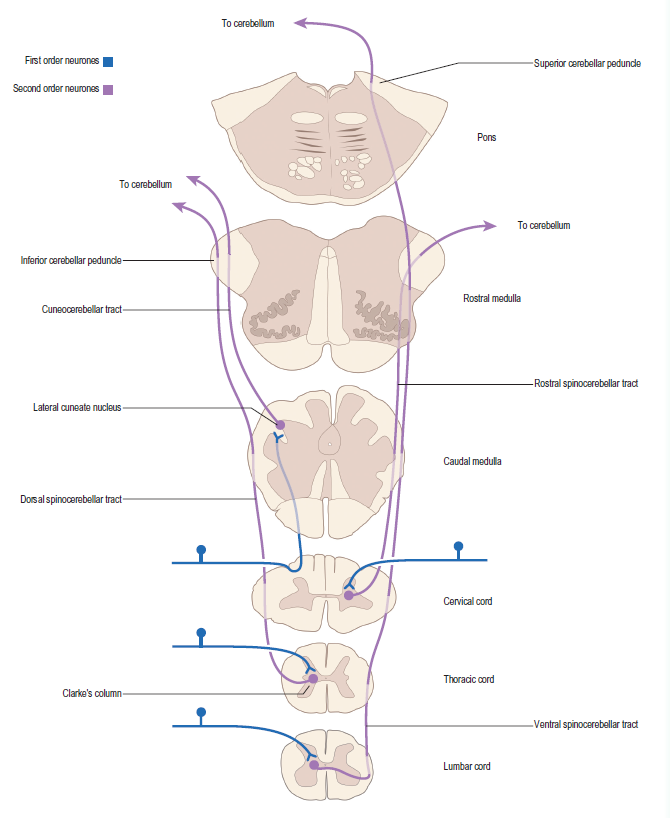
\includegraphics[width=0.85\textwidth]{pictures/Bilder_Laura/spinocerebellar_tract.PNG}
    \caption[Tractus spinocerebellaris]{\textbf{Tractus spinocerebellaris.} Vier unterschiedliche Bahnen werden dem Tractus spinocerebellaris zugeteilt. Der dorsale und ventrale spinocerebellare Trakt leiten Informationen aus den unteren Extremitäten an das Kleinhirn. Der dorsale Strang zieht ipsilateral im dorsolateralen Bereich des Rückenmarks nach oben. Der ventrale Trakt kreuzt auf die contralaterale Seite und steigt ventrolateral im Rückenmark auf. Das Äquivalent dieser Bahnen zu den oberen Extremitäten sind der rostrale spinocerebellare und der cuneocerebellare Trakt. Der cuneocerebellare Strang steigt ipsiliateral als Teil des Fasciculus cuneatus nach oben und projiziert dann über den Nucleus cuneatus in das Cerebellum. Die Axone des rostralen spinocerebellaren Strangs ziehen ipsilateral im Seitenstrang des Rückenmarks zum Kleinhirn. \\
    Abbildung aus \textit{Neuroanatomy}, Crossmann und Neary \textsuperscript{\cite[8]{crossman2014neuroanatomy}}.}
    \label{fig:tr_spinocerebellaris}
\end{figure}

\begin{figure}[H]
    \centering
    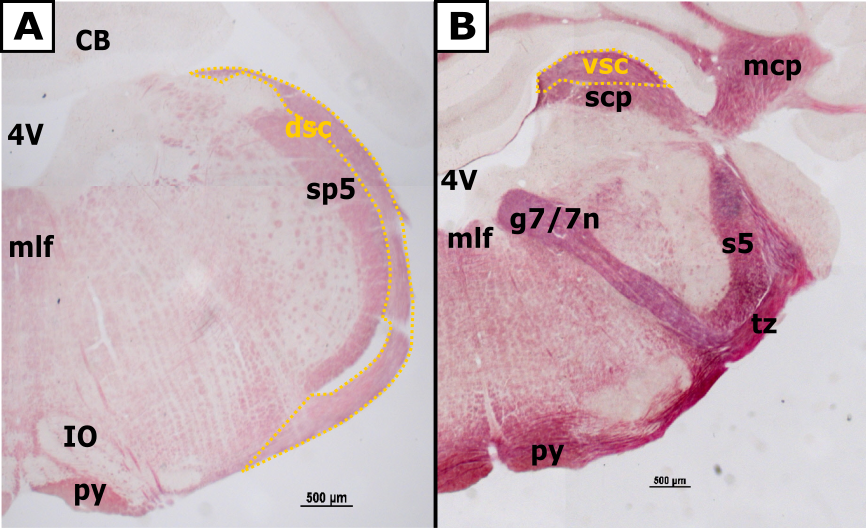
\includegraphics[width=0.7\textwidth]{pictures/Bilder_Laura/spinocerebellar_tract_F04_2P_025x_F09_1P_025x.png}
    \caption[Tractus spinocerebellaris Querschnitt]{\textbf{Tractus spinocerebellaris Querschnitt.} \textbf{A:} Der dorsale Tractus corticospinalis (dsc) zieht lateral des Hirnstamms entlang zum Cerebellum (CB). Unterhalb des vierten Ventrikels (4V) zieht sich der Fasciculus longitudinalis medialis (mlf) durch den Hirnstamm. Oberhalb der Pyramidenbahn (py) ist der untere Olivenkern (IO) zu erkennen. Seitlich des Hirnstamms ist der spinale Trakt des Trigeminusnerv (sp5). Faser-Färbung (F04-2). \textbf{B:} Der ventrale Tractus corticospinalis (vsc) ist hier zu erkennen, wie er über den superioren Kleinhirnstiel (scp) in das Cerebellum zieht.  Unterhalb des vierten Ventrikels (4V) zieht sich der Fasciculus longitudinalis medialis (mlf), der Nervus fascialis (7n) und das Knie des Nervus fascialis (g7) durch den Hirnstamm. Lateral lassen sich außerdem der mittlere Hinrstiel (mcp), der Trapezkörper (tz) und die sensorische Wurzel des Nervus trigeminus (s5) ausmachen. Ventral ist der Pyramidentrakt (py) zu sehen. Faser-Färbung (F09-1).}
    \label{fig:spinocerebellar}
\end{figure}
